\epigraph{\emph{
  ``Coming up with features is difficult, time-consuming, requires expert knowledge. "Applied machine learning" is basically feature engineering.''
}}{ Andrew Ng }

Considering the ``right'' features for clustering is a demanding and error prone process. Currently there is really just one way of describing documents: The vector space model. It breaks down to counting occurences and cooccurences of words and measuring distance by mathematical functions. We could just take all the words of a document, removing stopwords, and put them into a feature vector. This results in dimensionality explosion and extreme noise. Contrary to a document vector $d = \{w_1,w_2..w_n\}$, the feature vector represents a document by concepts $\{c_1,c_2,..c_j\}$. It is a projection of the original document $d = \{w_1,w_2..w_n\}$ to more general concepts resulting in fewer dimensions. This lifting is bestly described as combining several words of a document, often occuring in the same sentence, extracting a shared meaning. We hope to find fewer words that share enough information with the original word, that the following holds:
  
  \begin{equation}
    f : d=\{w_1,w_2,..w_n\} \to \{c_1,c_2,..c_j\}
  \end{equation}

The function $f$ transforms a sequence of words $w_1..w_n$ of a document $d$ to a sequence of concepts $c_1..c_j$. The concepts can be derived in a lot of ways.

  \begin{enumerate}
    \item Pruning words of low and high significance.
    \item Using syntactic parsing to retrieve noun phrases, named entity tags or part of speech tags.
    \item Using ontologies of \wordnet{} to derive a shared meaning of words.
    \item Mapping documents to \wiki{} categories.
    \item Using kernel methods (constrained clustering), preselecting initial clusters in a semi-supervised way.
  \end{enumerate}

In the end, feature selection is probably the most demanding task. Expert knolwedge needs to be applied and can change over time, called time drift. A computer handles documents in vector space, by counting. A human however perceives content differently. For any sufficiently adavanced algorithm that works with a knowledge base it is still: Garbage in, garbage out. More fancy algorithms will lead to better results, but better features will accelerate the accuracy.\\

In the following we will briefly explain what \emph{semantics} mean, especially in the \emph{domain} of newspapers. How \emph{feature selection} generally works and how this can be enhanced by \emph{syntactic parsing}. Strategies using \wordwiki{} are explained. In the experimental chapter we will then present how all these mechanisms come together.


\section{Semantics}
\label{sec:semantics}
  
  Semantics is the study of meaning. Given some symbols, characters, words or phrases what is their underlying meaning? The question is inherently hard and lots of literature focuses on how computers can get better at this. Most of the concepts depicted here taken from \cite{NLPBookJurafsky2000}. Semantics can also be viewed from a statistical point of view. Given a lot of phrases and words, can we infer their underlying structure that generated them? How can statistical patterns reveal what was meant and to what degree?\\
  In computational linguistics we often speak of \emph{word-sense disambiguation (WSD)}. \emph{WSD} is short for identifying sense of a word, if a word can have several meanings, in a sentence or paragraph. The sentence\\ 

    \emph{``The bail out during the financial crisis of the Lehmann brothers bank, was much too late.''}\\

  makes it obvious that it is about financial institutions ``bank'' during the financial crisis, political intervention by providing money ``bail out'' and a specific financial institution or entity ``Lehmann brothers''. How could we possibliy discern such a sentence so that we can actually reveal all the beforementioned concepts? To successfully find such concepts we have to identify what parts of speech, e.g. nouns, verbs, adjectives etc., each word of a document has:

    \begin{equation}
      pos\-tag(d=[w_1,w_2,..w_n]) = [(w_1, tag_1), (w_2, tag_2),.. (w_n, tag_n)]
    \end{equation}

  Part of speech tagging works by parsing a document sentence by sentence. Tagging each word by identifying its position relative to other words and predicting what their tags might look like. See \cite[chp. 5]{NLPBookJurafsky2000} for an extensive study.
  For clustering we want to identify these \emph{semantic fields}, a set of words grouped by meaning. We then often analyze \emph{WSD} through \emph{synonymy, polysemy, hyponymy, hypernymy and meronymy}. All of those concepts are important to taxonomies and ontologies. A \emph{taxonomy} is refered to as a simple hierarchical structure of parent-child relationships, that change in granularity per hierarchy level. An \emph{ontology} is much broader and can have complex relations other than parent-child. In that sense both taxonomies and ontologies are structures, showing how to classify words in context to each other. Traversing through these hierarchical structures is typically done by hyponyms and hypernyms. 

    \begin{figure}[h!]
      \centering
        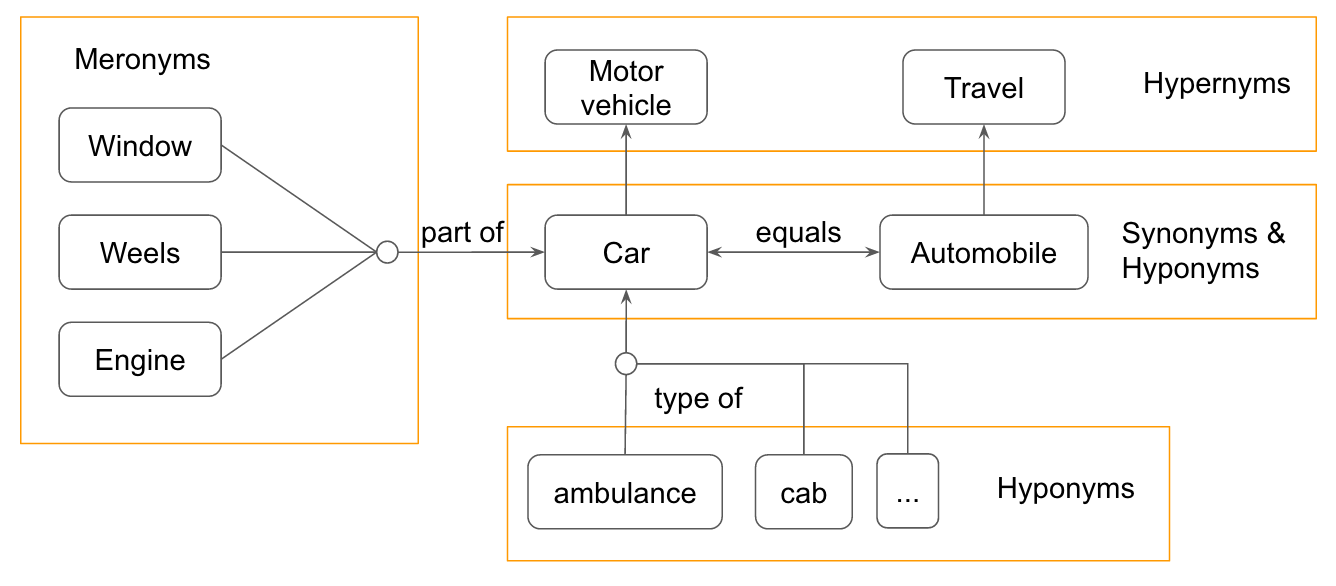
\includegraphics[width=0.9\textwidth]{wsd_analysis.png}
        \caption{"Semantic fields, hierarchies"}
        \label{wsd_analysis}
    \end{figure} 

  \emph{Meronyms} are ``part-of'' relations, \emph{hyponyms} have a ``type-of'' relation to a higher concept, called \emph{hypernyms}. In figure \ref{wsd_analysis} we see that from a single concept ``car'' we can infer a semantic field around it. We will see later how this works, a statistical concept around this is \emph{LSI} and \emph{probabilistic topic modelling}. The symbolic way is to use knowledge bases such as \wordwiki{}.\\

  In the text \emph{domain} of newspaper articles a few problems arise. Analyzing a long book, a long speech or journal articles from the scientific community, is easier compared to high varying fragments from different authors on different topics. A long book written by one person will use a specific language that is typical of that author. Speeches for a specific person contain similar concepts and often use the same language as well. In the scientific community rhethorial and anecdotal phrasing is uncommon. Facts, citation and correct formatting is of central importance. The text might be heterogenous but the fact remains that a certain wording / glossary, is shared throughout these examples.\\

  This does not hold true for newspaper articles. \emph{Topics} about different events co-occuring on the world. Different \emph{authors} with different writing styles. Different \emph{newspapers} with different directions of content presentation. \emph{Long} and very \emph{short} articles. And this does not take images, videos or comments into account. When dealing with a vast landscape of different topics, spanning connections between two documents becomes a hard task. In context of such sparse data, that is documents with almost no connecting words, clustering works poorly. This can also be described as a high variance problem, where each document contributes a lot of unseen words to the feature vector.\\

  In order to avoid these variance problems, we need to find a solution to \emph{WSD} and then apply a lifting from the original concept to a hypernym. Going back to figure \ref{wsd_analysis} we see that \emph{car} and \emph{motored vehicle} might mean the same thing. Both are about cars, if we project the concept \emph{car} to \emph{motored vehicle} the concept would connect both the documents containing car and motored vehicle. This is not always what we want to achieve but it could drastically improve similarity between documents that would miss each other by synonymy and polysemy.

\section{Selection}
\label{sec:selection}

  As described before we want to tackle \emph{WSD} and find ways to connect documents that share common meaning but not a lot of common words. To do so we have several strategies at our disposal. First, word pruning is presented, it is probably the most widely used technique for lowering dimensions and removing insignificant words. Second, synctactic parsing is described in by part of speech tagging, noun phrase extraction and named entity recognition. One topic which is left out are the kernels. They are important to retrieve better results in a semi supervised way but could not make it into the thesis experiments.

  \subsection{Word pruning}
  \label{sec:word_pruning}

    Before pruning words we have to convert the documents into a suitable vsm such as \emph{counting vectors} or \emph{TF-IDF} described in \ref{sec:bag_of_words}. The counting alone in its basic form is sufficient in telling if a term has a high or low connection with all other documents. The \emph{TF-IDF} on the other hand is a measure of importance and solely based on the resulting frequencey per word. It is possible to make significant pruning on both representations. The \emph{TF-IDF} variant is prefered as it normalizes frequencies. Higher or lower counts are weighted into a formula that better represents the significance of a term.\\

    Either way we need to create a cooccurence matrix $M = count(C, D)$ where $C$ is a corpus and $D$ is the dictionary of the corpus. Then we transform by $M = tfidf(M)$ or leave it with the \emph{term frequency}.\\

    Pruning $M$ is done by cutting off the documents with a very low ratio of counts with respect to all documents. This can be done by threshold in proportion to all terms, a percentage, removing $j$ terms. It can also be achieved by a hard count, cutting of all terms that have no counts higher than that. This means, we remove insignificant terms or terms that do not contribute to any connection. Semantically this means, we cut off words that have a high meaning in a single document and a very low in others. Those words are redundant, or in other words they have no discriminant value to the clustering process.

      \begin{equation}
      \begin{split}
        m &= [0, 1, 5, 0, 4, 0, 1, 1, 2, 3] \\
        m_s &= sort( [0, 0, 0, 1, 1, 1, 2, 3, 4, 5] ) \\
        percentcut(m_s, 0.2) &= [0, 1, 1, 1, 2, 3, 4, 5] \\
        totalcut(m_s, 1) &= [2, 3, 4, 5]
      \end{split}
      \end{equation}

    The min cut on percentage $0.2 = 20\%$ cuts the first 2 samples or removes the first 6 in case of a total count. The parameter has to be varied, depending on the outcome of a cost function. Further we can take off the top $j$ words as well by the same principle. The problem with the top words is, that they highly correlate with a lot of different documents, meaning a high correlation between a term and the corpus. Leaving them out erases a lot of connections, resulting in more discriminant features. This is what we want to achieve, finding the middle words, that are common in certain documents and uncommon in others. During clustering this will result in much more coherent clusters.

      \begin{equation}
      \begin{split}
        m &= [0, 1, 5, 0, 4, 0, 1, 1, 2, 3] \\
        m_s &= sort( [0, 0, 0, 1, 1, 1, 2, 3, 4, 5] ) \\
        maxcut(m_s, 0.8) &= [0, 0, 0, 1, 1, 1, 2, 3]
      \end{split}
      \end{equation}

    The max cut works with a ratio that selects from lowest to highest 80\% except the last 20\%. Note that the samples are not on $m$ dimensional vectors. For this to work we have to aggregate the counts and then prune the most insignificant words. The great thing of this approach is that it can follow any feature selection strategy. By using word pruning on feature vectors, the selection process can be refined. The fine tuning is necessary in gaining percentages in accuracy.

  \subsection{Syntactic parsing}
  \label{sec:syntactic_parsing}

  Parsing reduces symbols, to a parsed tree of following expressions. In English parsing, probabilistic shift reduce parsers in combination with trained neural networks is state of the art. \cite{ShiftReduceParsingStanford} Valid words and characters are defined within the rules of the English alphabet. In figure \ref{syntactic_parsing} we can see a parse tree for an English sentence parser. The parsing is syntactical based on English grammar. When it comes to parsing expressions from English language to a meaningful representation for the computer, the problem statement gets a lot more difficult. Too many words, too many forms of sentences - statistics in combination with structural parsers come to the rescue. Solely syntactic parsers that work on symbols work well in a specific domain up to a certain parsing accuracy. Statistical models remove these barriers by likelikhoods and predictions, finding answers accross domains. The most inherent problem is overfitting. Overfitting describes that a probabilistic parser works well on a specific problem domain or data source, because it learned the domain well. Unseen domains and datasets perform poorly due to the missing knowledge. The problem becomes more clear, in the domain of newspaper articles where different language styles and domains are frequent. Statistical parsers like the \emph{Stanford} parser are very accurate in identifying valid syntactic English expressions. In the following we will look more closely at noun phrase extraction and named entity recognition. They can be used as initial seeds for the feature space of a corpus.

    \begin{figure}[h!]
      \centering
        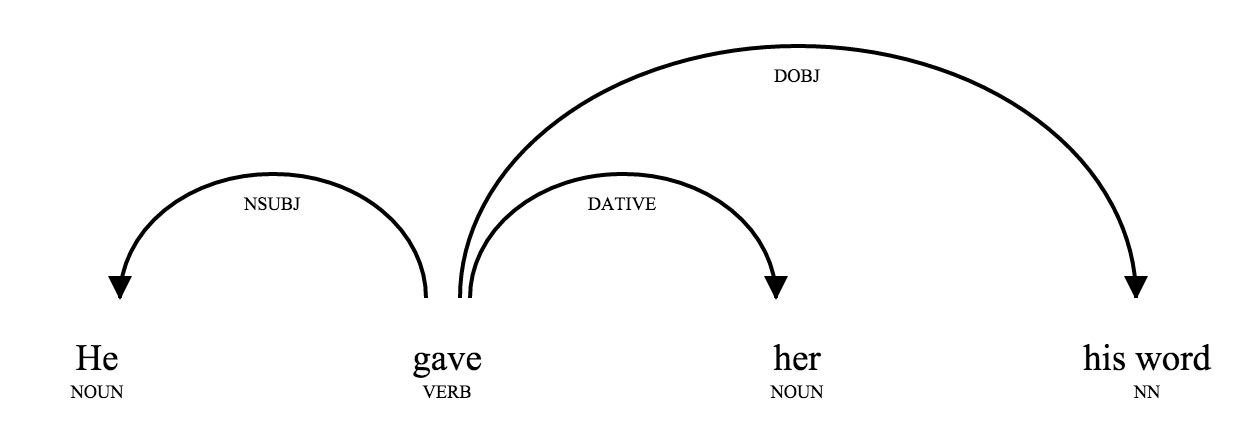
\includegraphics[width=0.9\textwidth]{sentence_structure.png}
        \caption{"Syntactic parsing"}
        \label{syntactic_parsing}
    \end{figure} 

  Figure \ref{syntactic_parsing} is displayed as a projective tree, where each word has exactly one (or none) incoming and outgoing edge. The outgoing edge is refered to as head. Edges contain information about the relation between both words. Each word has a part of speech tag described by many corpuses. Current research projects use Googles ngrams over time, with a 3 billion ngram corpus to infer the most likely structures. \cite{SyntacticNgramsOverTime2013}
  The parsing of English grammatical structures is entirely dependant upon specification of the rules. What part of speech tagging system is used? How is the grammar defined? With the help of the Chomsky hierarchy it was proven that not all natural languages have context-sensitive (type-1) nor turing complete (type-0) grammars. See \cite[chp. 16]{NLPBookJurafsky2000} for a great introduction.
  In clustering this is not a huge problem, because the granularity of the task is not that fine tuned. A slightly false parse might still yield good feature results.

  \subsubsection*{Noun phrases}
  Noun phrases are often referred to as key phrases. Formally a noun phrase is a phrase with a noun as its head word. A head is a word that determines the syntactic type of a phrase. Generally a noun phrase is a part of a sentence that captures meaning of a sentence. Thusly they are good samples to represent a document. However noun phrases are rather bad samples for clustering. They do not connect well to other documents due to their unique occurences. In the \wordnet{} section we will see how they are great for projecting to their respective hypernyms. Noun phrase extraction is highly connected with part of speech tagging where certain tag patterns are used to filter nouns or noun phrases. For further information see \cite[chp. 5, 12]{NLPBookJurafsky2000}.

  \subsubsection*{Named entities}
  Named entity recognition is the task of information retrieval that extracts and classifies  names of persons, organizations, locations, expressions of times, quantities, monetary values, percentages, etc. \cite[chp. 22]{NLPBookJurafsky2000}. 

    \begin{figure}[h!]
      \centering
        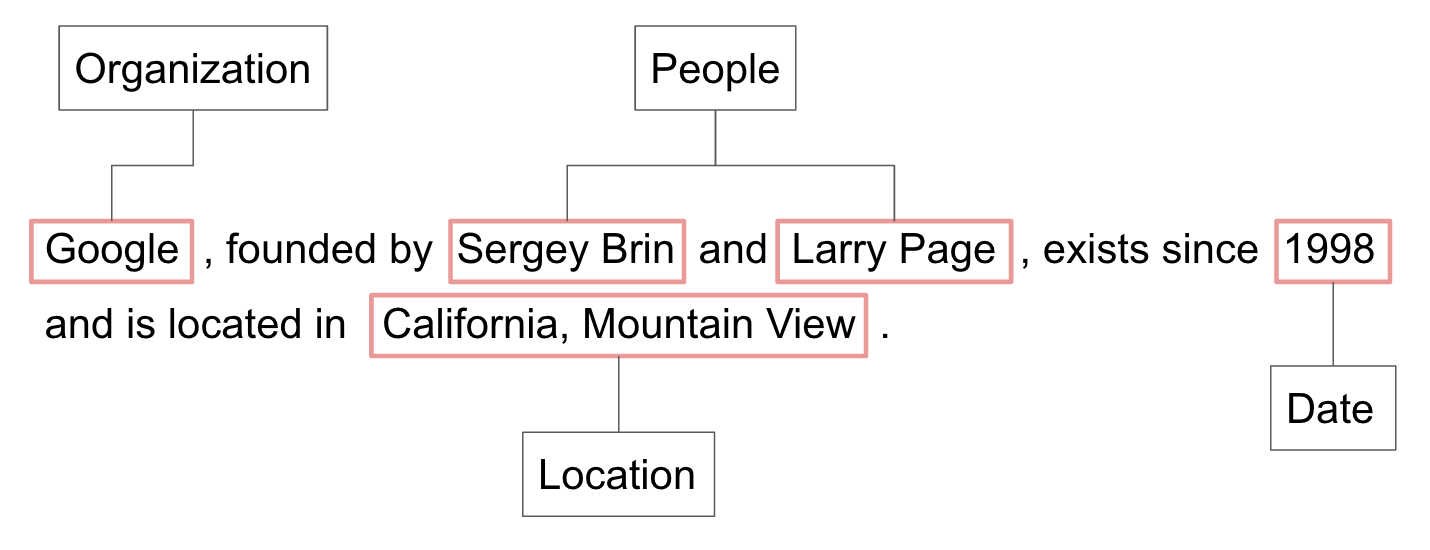
\includegraphics[width=0.9\textwidth]{ner_tags.png}
        \caption{"Named entities"}
        \label{ner_tags}
    \end{figure} 

  As seen in figure \ref{ner_tags} we are interested in informative terms. Often occuring named entities tend to give a direction what a document is about. If Google occurs in one document, it most likely will have to do with a lot of other documents that are about Google. We would like to favor documents that are connected by their respective named entities and weight them in more than others. Named entities like noun phrases are very discriminative. In systems like the Columbia Newsblaster system, named entities would be used to determine if a document is biographical, has large shifts in time (dates) or connecting documents based on significant organizations, peoples etc. \cite{ColumbiaMultiDoc2001}

\section{External Knowledge}
\label{sec:semantic_selection}

  In order to enhance the syntactical selection models we can add a knowledge base such as \wordwiki{}. The data reresentation is often defined as a typical dictionary. For a definition of a word we can infer semantic fields and additional text describing the words in more detail. Moreover knowledge bases such as \wiki{} categorize/classify concepts into ontologies. \wordwiki{} are great in the sense that human authors around the world add missing information and enhance the models frequently. The knowledge bases are enhanced frequently by writing rules and reviewing processes.

  \subsection{WordNet}
  \label{sec:wordnet}

  \wordnet{} is a lexical database of English. Lexical parts of speech such as nouns, verbs or adjectives are grouped into synonyms (synsets). Each synset is linked by semantical and lexical relations. In parts \wordnet{} resembles a thesaurus, grouping words based on meaning. With its onotologies it deals with \emph{WSD}. Further words are interlinked by semantic relations. For more information see \cite{Wordnet1995, Wordnet1998}. \\
  \wordnet{} is often used for lemmatization. Lemmatization is the process of removing the inflected forms of a given word to its lemma. A lemma is a dictionary entry or canonical form of a word. The major difference to stemming is that \wordnet{} is able to inflect a canonical form that depends on context sensitive pos tags. 

    \begin{equation}
    \begin{split}
      lemmatize("savings", pos="noun") &\to "saving" \\
      lemmatize("savings", pos="verb") &\to "save" \\
      stem("savings") &\to "save" \\
      stem("save") &\to "save"
    \end{split}
    \end{equation}

  Inflecting the canonical form with pos tags enhances the precision of the context where the words came from. Often this can result in different inflectional forms that would otherwise be equal. In comparisson we can see that stemming treats ``savings'' and ``save'' entirely the same. This is a basic strategy to inflect a generalized version of a document, to lower the dimensions. Further we can take the hypernyms of a document.

    \begin{equation}
    \begin{split}
      \sum_{i=1}^{|d|} hypernyms_{first}(d_i)
    \end{split}
    \end{equation}

  We iterate over all words in $d$ and take the first of the hypernyms of the words, projecting it to a higher concept. \wordnet{} sorts the hypernyms from most likely to less likely, taking the first is a good approximation.
  Enhancing the above statement we scale this up to the depth $d$ going up the hypernyms of the \wordnet{} ontologies.

    \begin{equation}
    \begin{split}
      closure(seq, d=0) &= empty \\
      closure(seq, d>0) &= \sum_{w \in seq} closure(hypernyms(w), d-1)
    \end{split}
    \end{equation}

  At last, we can infer the most common meaning of a sentence by calculating the lowest common hypernyms. 

    \begin{equation}
      lowest\_common\_hypernyms(w_1, w_2) = hypernyms(w_1) \cap hypernyms(w_2)
    \end{equation}

  For this we compute for each word in a document the transitive closure with the above statement not restricted by the first hypernym.

    \begin{algorithm}[H]
    \begin{algorithmic}[1]
      \caption{\wordnet{} closure with hypernyms}\label{wordnet}
      \For{$sent \in closure(doc, d)$}
        \For{$(w_1, w_2) \in sent : w_1 \not = w_2$}
          \State $result \gets lowest\_common\_hypernyms(w_1, w_2)$
        \EndFor
      \EndFor
      \State \Return $result$
    \end{algorithmic}
    \end{algorithm}

  Then we compute the lowest common hypernyms that connect hypernyms of the word closures. We then apply word pruning to get the mid vector words, sorting out extremes. It is also possible to greatly enhance the above models with lexical chains, see \cite{SemanticClusteringWithWordnet}.

  \subsection{Wikipedia}
  \label{sec:wikpedia}
    

